\documentclass[12pt]{article}
\usepackage{amsmath, amssymb, amsthm, graphicx, geometry, listings, xcolor, url, enumitem, fancyhdr, multirow}
\geometry{margin=1in}
\definecolor{darkgreen}{rgb}{0,0.5,0}
\pagestyle{fancy}

\lstset{
    frame=tb,
    language=Python,
    aboveskip=3mm,
    belowskip=3mm,
    showstringspaces=false,
    columns=flexible,
    basicstyle={\small\ttfamily},
    numbers=none,
    numberstyle=\tiny\color{green},
    keywordstyle=\color{blue},
    commentstyle=\color{darkgreen},
    stringstyle=\color{orange},
    breaklines=true,
    breakatwhitespace=true,
    tabsize=3
}

\lhead{SFSU, CSC 671-01}
\chead{Spring 2025}
\rhead{Deep Learning}

\title{Multi-Layer Perceptron for Non-Linear Regression}
\author{Bryan Lee\\922649673}
\date{March 8, 2025}

\begin{document}

\maketitle
\thispagestyle{fancy}

\section{Introduction}
This project focuses on implementing a Multi-Layer Perceptron (MLP) for non-linear regression, with the goal of predicting continuous values based on input data.
Unlike classification models that assign discrete class labels, regression models generate numerical predictions that capture complex, non-linear relationships within the data.
The objective is to train a basic MLP to learn a function that effectively maps x to y, identifying the underlying pattern in the dataset.
Since this is a regression task, Softmax and Argmax activation functions, commonly used for classification, are unnecessary.
Instead, the model outputs a single continuous value, representing the result of the learned non-linear function.

\section{Data}
The dataset used for this project consists of 1,000 data points, where x represents the independent (predictor) variable and y is the dependent (response) variable.
Using a linear regression would yield a straight line-of-best fit; however, it fails to capture the relevant discrepancy and patterns in the data.
To achieve our objective, an MLP model with hidden layers and non-linear activation functions can effectively capture the complex patterns and provide a non-linear fit to the data.

\begin{figure}[ht]
    \centering
    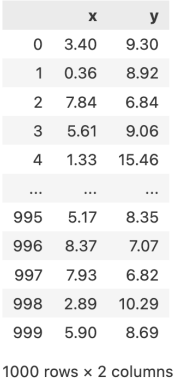
\includegraphics[width=0.2\linewidth]{DataSet.PNG}
    \caption{The provided dataset.}
\end{figure}

\newpage

\section{MLP Class}
The MLP model that fits the data the best consists of four connected layers: three hidden layers and one output layer.
The input to the first layer is x, which is normalized and reshaped to a 2D tensor during pre-processing.
The hidden layers use ReLU activation functions, while the output layer produces a single continuous value without activation.
The best architecture (creating a smooth curve) for the MLP model is as follows:

\begin{itemize}
    \item Hidden Layer: 1 $\rightarrow$ 400 neurons, ReLU activation
    \item Hidden Layer 2: 400 neurons $\rightarrow$ 250 neurons, ReLU activation
    \item Hidden Layer 3: 250 neurons $\rightarrow$ 80 neurons, ReLU activation
    \item Output Layer: 80 neurons $\rightarrow$ 1 neuron
\end{itemize}

\section{Data Preprocessing}
As the data is not centered around zero, it is normalized using z-score standardization to origin (0, 0).
Normalization ensures that all features have similar magnitudes.
The data normalization process is as follows:

\begin{itemize}
    \item Compute the mean and standard deviation for both x and y.
    \item Normalize x and y using the z-score standardization formula:
        \begin{equation*}
            x_{norm} = \frac{x - \mu_x}{\sigma_x},\quad y_{norm} = \frac{y - \mu_y}{\sigma_y}
        \end{equation*}
\end{itemize}

After training, the model's prediction will be denormalized for plotting via:

\begin{equation*}
    Y_{\text{denorm}} = f\left(\frac{X - \mu_X}{\sigma_X}\right) \cdot \sigma_Y + \mu_Y
\end{equation*}

\section{Training Process}
The MLP is trained using the Mean Squared Error (MSE) loss and the Adam optimizer.
The training process takes in the provided data loader, calculates the loss, and adjusts the weights through backpropagation.
The training loop is as follows:

\begin{enumerate}
    \item For each epoch:
        \begin{itemize}
            \item Reshape feature and label to 2D tensors.
            \item Perform forward propagation to compute the predicted values.
            \item Compute the MSE loss between the predicted and true values. The MSE loss function is defined as:
                \begin{equation*}
                    \text{MSE} = \frac{1}{N} \sum_{i=1}^N (y^{[i]} - \hat{y}^{[i]})^2
                \end{equation*}
            \item Perform backward propagation to compute gradients.
            \item Update the weights using the Adam optimizer.
        \end{itemize}
    \item Track the loss at each epoch.
\end{enumerate}

\section{Hyper-Parameters Search}
The hyperparameters explored for the MLP model are as follows:
\begin{enumerate}
    \item Batch Size: [32, 64, 128]
    \item Learning Rate: [0.01, 0.001, 0.0001]
    \item Number of Epochs: [25, 50, 100]
\end{enumerate}


\noindent Each combination of hyperparameters is evaluated via the training process and the loss is recorded.
Before the training process, the normalized data is placed into a data loader with the specified batch size and shuffled.
The combination with the less loss is selected as the best hyperparameters.

\section{Results}
After training the MLP, there were varying results; however, two hyperparameter combinations gave a fairly smooth and closely approximated regression curve. \\

\noindent The 2nd best hyperparameters:
\begin{itemize}
    \item Batch Size: 64
    \item Learning Rate: 0.001
    \item Number of Epochs: 100
    \item Activation Function: ReLU
    \item Optimizer: Adam
    \item Number of Layers: 4
    \item Number of Neurons per Layer: 400, 250, 80, 1
\end{itemize}

\begin{figure}[ht]
    \centering
    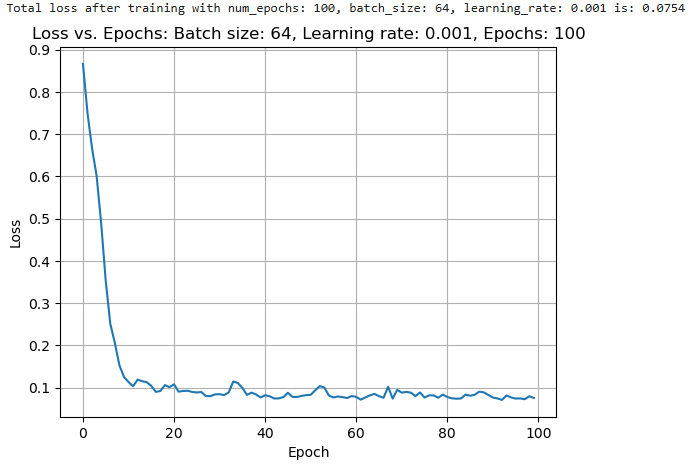
\includegraphics[width=0.9\linewidth]{Loss2ndBest.PNG}
    \caption{Training loss for the 2nd best hyperparameters.}
\end{figure}

\newpage

\begin{figure}[ht]
    \centering
    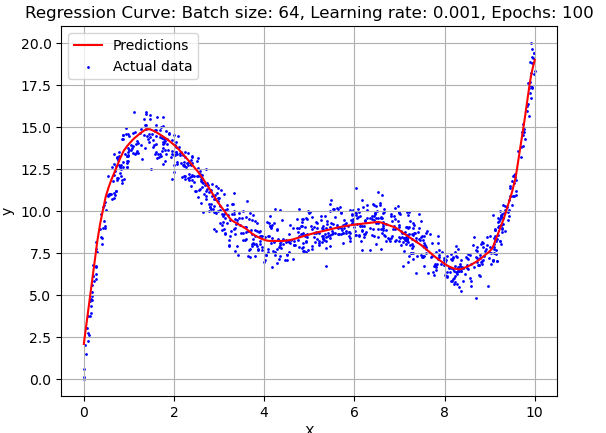
\includegraphics[width=0.9\linewidth]{RegressionCurve2ndBest.PNG}
    \caption{Regression curve for the 2nd best hyperparameters.}
\end{figure}

\noindent The best hyperparameters:
\begin{itemize}
    \item Batch Size: 128
    \item Learning Rate: 0.001
    \item Number of Epochs: 100
    \item Activation Function: ReLU
    \item Optimizer: Adam
    \item Number of Layers: 4
    \item Number of Neurons per Layer: 400, 250, 80, 1
\end{itemize}

\newpage

\begin{figure}[ht]
    \centering
    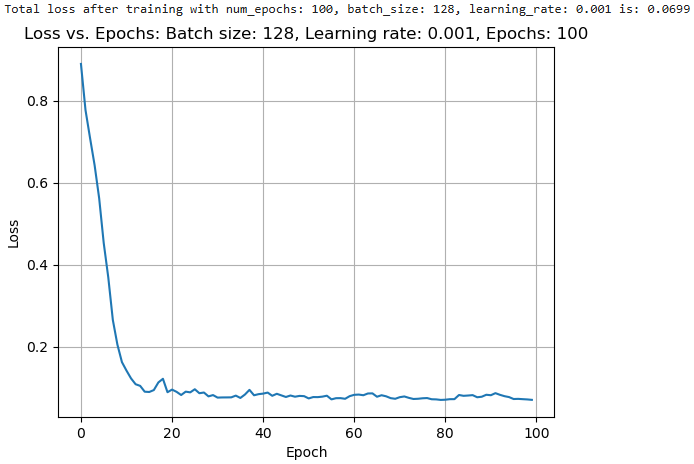
\includegraphics[width=0.9\linewidth]{BestLoss.PNG}
    \caption{Training loss for the best hyperparameters.}
\end{figure}

\newpage

\begin{figure}[ht]
    \centering
    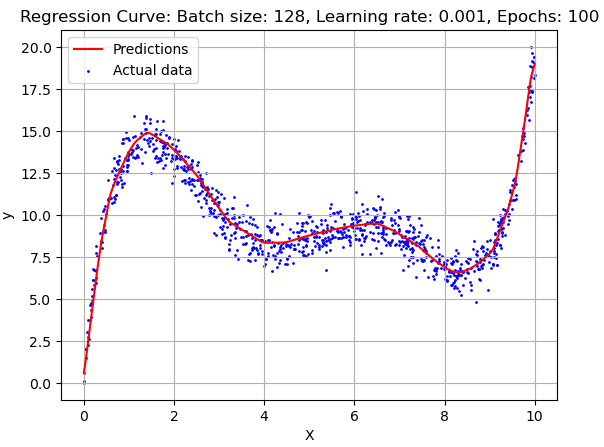
\includegraphics[width=0.9\linewidth]{BestRegressionCurve.PNG}
    \caption{Regression curve for the best hyperparameters.}
\end{figure}

\section{Conclusion}
While a larger data size and higher learning rate might seem to offer the best approximation, the results do not necessarily support this assumption.
The difference between the second-best hyperparameters and the best ones is only about 0.55 percent.
Several factors influence the choice of the best model, such as prioritizing performance over accuracy or considering different data sizes.
In conclusion, the model could be further optimized with a more complex architecture, additional data, and more epochs; however, the improvements would likely be marginal compared to the significant increase in training time.

\end{document}
